\documentclass[a4paper, 12pt]{article}
\date{27 February 2014}
\author{Shaun Schreiber \\ 16715128}
\title{Tutorial 2}
\usepackage{float}
\usepackage{tikz}
\usepackage{graphicx}
\usetikzlibrary{arrows, automata}
\begin{document}
\maketitle
\section*{Question 4a}
\begin{figure}[H]
\minipage{0.32\textwidth}
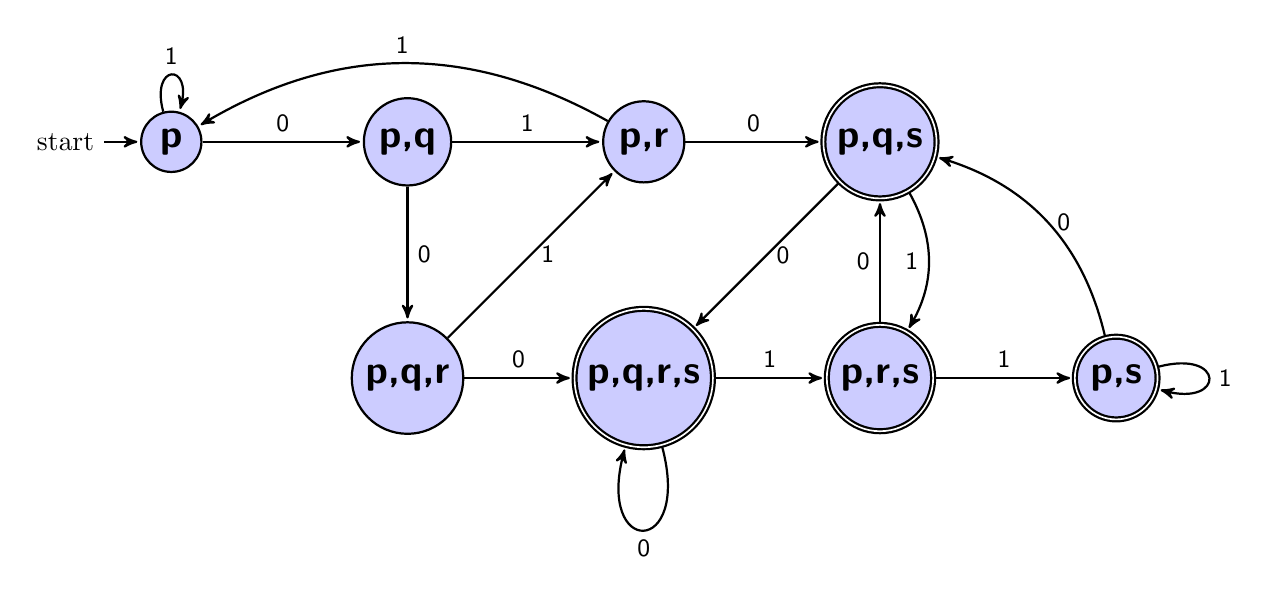
\begin{tikzpicture}[->,>=stealth',shorten >=1pt,auto,node distance=3cm,
  thick,main node/.style={circle,fill=blue!20,draw,font=\sffamily\Large\bfseries}]
  \node[main node, initial] (p) {p};
  \node[main node] (pq) [right of =p] {p,q};
  \node[main node] (pqr) [below of =pq] {p,q,r};
  \node[main node] (pr) [right of =pq]{p,r};
  \node[main node, accepting] (pqrs) [right of =pqr]{p,q,r,s};
  \node[main node, accepting] (pqs) [right of =pr] {p,q,s};
  \node[main node, accepting] (prs) [right of =pqrs] {p,r,s};
  \node[main node, accepting] (ps) [right of =prs] {p,s};
  \path[every node/.style={font=\sffamily\small}]
     (p)    edge[loop above] node [above]{1}(p)
	    edge node [above]{0}(pq)
     (pq)   edge node[above] {1}(pr)
            edge node [right] {0}(pqr)
     (pr)   edge[bend right] node [above]{1}(p)
	    edge node [above]{0}(pqs)
     (pqr)  edge node [right]{1}(pr)
	    edge node [above]{0}(pqrs)
     (pqrs) edge node [above]{1}(prs)
	    edge [loop below] node [below]{0}(pqrs)
     (pqs)  edge [bend left] node [left] {1} (prs)
            edge  node [right]{0}(pqrs)
     (prs)  edge node [above]{1}(ps)
	    edge node [left]{0}(pqs)
     (ps)   edge [loop right] node [right]{1}(ps)
	    edge [bend right] node [right]{0}(pqs);       
  \end{tikzpicture}
\endminipage\hfill
\end{figure}
\begin{table}[h!t]
\centering
\begin{tabular}{c | c c}
& 0 & 1 \\
\hline
\{$p$\} & \{$p, q$\} & \{$p$\} \\
\{$p, q$\} & \{$p, q, r$\} & \{$p, r$\} \\
\{$p, q, r$\} & \{$p, q, r, s$\} & \{$p, r$\} \\
\{$p, r$\} & \{$p, q, s$\} & \{$p$\} \\
\{$p, q, r, s$\} & \{$p, q, r, s$\} & \{$p, r, s$\} \\
\{$p, q, s$\} & \{$p, q, r, s$\} & \{$p, r, s$\} \\
\{$p, r, s$\} & \{$p, q, s$\} & \{$p, s$\} \\
\{$p, s$\} & \{$p, q, s$\} & \{$p, s$\} \\
\end{tabular}
\end{table}\section*{Question 4b}
\begin{figure}[H]
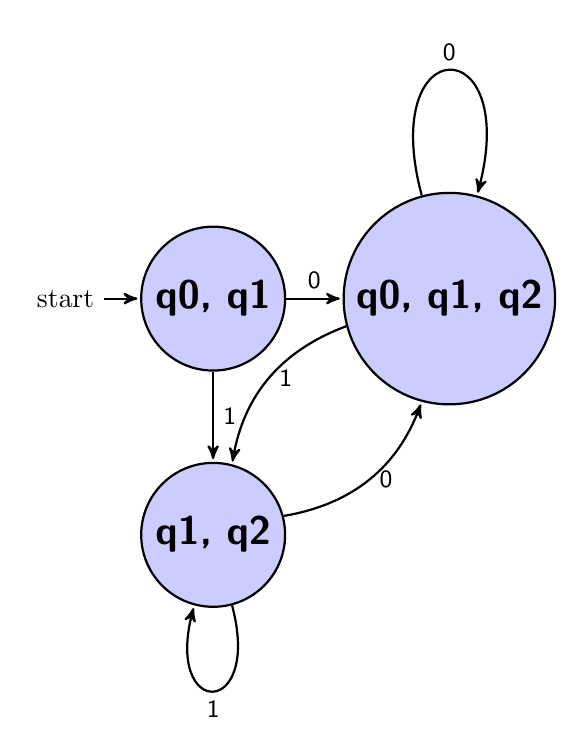
\begin{tikzpicture}[->,>=stealth',shorten >=1pt,auto,node distance=3cm,
  thick,main node/.style={circle,fill=blue!20,draw,font=\sffamily\Large\bfseries}]
  \node[main node, initial] (q0q1) {q0, q1};
  \node[main node] (q0q1q2) [right of =q0q1] {q0, q1, q2};
  \node[main node] (q1q2) [below of =q0q1] {q1, q2};
  \path[every node/.style={font=\sffamily\small}]
     (q0q1)   edge node [right]{1}(q1q2)
              edge node [above]{0}(q0q1q2)
     (q0q1q2) edge [loop above] node [above] {0}(q0q1q2)
	      edge [bend right] node [right] {1}(q1q2)
     (q1q2)   edge [loop below] node [below] {1}(q1q2)
	      edge [bend right] node [right]{0}(q0q1q2);
  \end{tikzpicture}
\end{figure}
\begin{table}[h!t]
\centering
\begin{tabular}{c | c c}
& 0 & 1 \\
\hline
\{$q0, q1$\} & \{$q0, q1, q2$\} & \{$q1, q2$\} \\
\{$q0, q1, q2$\} & \{$q0, q1, q2$\} & \{$q1, q2$\} \\
\{$q1, q2$\} & \{$q0, q1, q2$\} & \{$q1, q2$\} \\
\end{tabular}
\end{table}
\section*{Question 5a}
\subsection*{a}
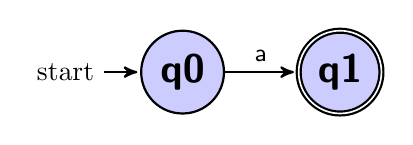
\begin{tikzpicture}[->,>=stealth',shorten >=1pt,auto,node distance=2cm,
  thick,main node/.style={circle,fill=blue!20,draw,font=\sffamily\Large\bfseries}]
  \node[main node, initial] (q0) {q0};
  \node[main node, accepting] (q1) [right of =q0] {q1};
  \path[every node/.style={font=\sffamily\small}]
     (q0) edge node [above]{a}(q1);
  \end{tikzpicture}
\subsection*{b}
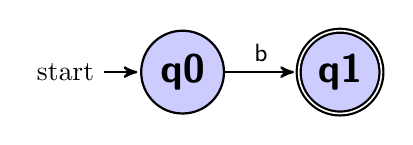
\begin{tikzpicture}[->,>=stealth',shorten >=1pt,auto,node distance=2cm,
  thick,main node/.style={circle,fill=blue!20,draw,font=\sffamily\Large\bfseries}]
  \node[main node, initial] (q0) {q0};
  \node[main node, accepting] (q1) [right of =q0] {q1};
  \path[every node/.style={font=\sffamily\small}]
     (q0) edge node [above]{b}(q1);
  \end{tikzpicture}
  \subsection*{b*}
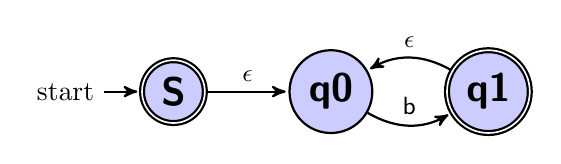
\begin{tikzpicture}[->,>=stealth',shorten >=1pt,auto,node distance=2cm,
  thick,main node/.style={circle,fill=blue!20,draw,font=\sffamily\Large\bfseries}]
  \node[main node, initial, accepting] (S) {S};
  \node[main node] (q0) [right of =S] {q0};
  \node[main node, accepting] (q1) [right of =q0] {q1};
  \path[every node/.style={font=\sffamily\small}]
     (S) edge  node [above]{$\epsilon$}(q0)
     (q0) edge[bend right] node [above]{b}(q1)
     (q1) edge [bend right] node [above]{$\epsilon$}(q0);
  \end{tikzpicture}
  \subsection*{a*}
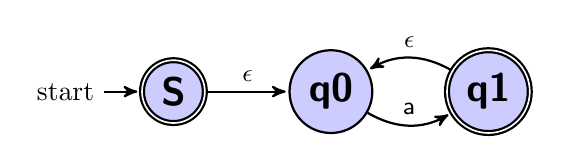
\begin{tikzpicture}[->,>=stealth',shorten >=1pt,auto,node distance=2cm,
  thick,main node/.style={circle,fill=blue!20,draw,font=\sffamily\Large\bfseries}]
  \node[main node, initial, accepting] (S) {S};
  \node[main node] (q0) [right of =S] {q0};
  \node[main node, accepting] (q1) [right of =q0] {q1};
  \path[every node/.style={font=\sffamily\small}]
     (S) edge  node [above]{$\epsilon$}(q0)
     (q0) edge[bend right] node [above]{a}(q1)
     (q1) edge [bend right] node [above]{$\epsilon$}(q0);
  \end{tikzpicture}
\subsection*{ab}
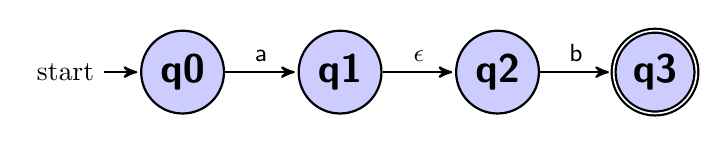
\begin{tikzpicture}[->,>=stealth',shorten >=1pt,auto,node distance=2cm,
  thick,main node/.style={circle,fill=blue!20,draw,font=\sffamily\Large\bfseries}]
  \node[main node, initial] (q0) {q0};
  \node[main node] (q1) [right of =q0] {q1};
  \node[main node] (q2) [right of =q1] {q2};
  \node[main node, accepting] (q3) [right of =q2] {q3};
  \path[every node/.style={font=\sffamily\small}]
     (q0) edge node [above]{a}(q1)
     (q1) edge node [above]{$\epsilon$}(q2)
     (q2) edge node [above]{b}(q3);
  \end{tikzpicture}
\subsection*{ab*}
\begin{tikzpicture}[->,>=stealth',shorten >=1pt,auto,node distance=2cm,
  thick,main node/.style={circle,fill=blue!20,draw,font=\sffamily\Large\bfseries}]
  \node[main node, initial,accepting] (S) {S};
  \node[main node] (q0) [right of =s ] {q0};
  \node[main node] (q1) [right of =q0] {q1};
  \node[main node,accepting] (q2) [right of =q1] {q2};
  \node[main node] (q3) [right of =q2] {q3};
  \node[main node, accepting] (q4) [right of =q3] {q4};
  \path[every node/.style={font=\sffamily\small}]
     (S)  edge node [above]{$\epsilon$} (q0)
     (q0) edge node [above]{a}(q1)
     (q1) edge node [above]{$\epsilon$}(q2)
     (q2) edge node [above]{$\epsilon$}(q3)
     (q3) edge [bend right] node [above] {b}(q4)
      (q4) edge [bend right] node [above] {$\epsilon$}(q3);
  \end{tikzpicture}
\subsection*{aa}
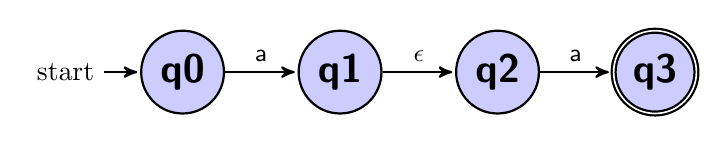
\begin{tikzpicture}[->,>=stealth',shorten >=1pt,auto,node distance=2cm,
  thick,main node/.style={circle,fill=blue!20,draw,font=\sffamily\Large\bfseries}]
  \node[main node, initial] (q0) {q0};
  \node[main node] (q1) [right of =q0] {q1};
  \node[main node] (q2) [right of =q1] {q2};
  \node[main node, accepting] (q3) [right of =q2] {q3};
  \path[every node/.style={font=\sffamily\small}]
     (q0) edge node [above]{a}(q1)
     (q1) edge node [above]{$\epsilon$}(q2)
     (q2) edge node [above]{a}(q3);
  \end{tikzpicture}
\subsection*{bba}
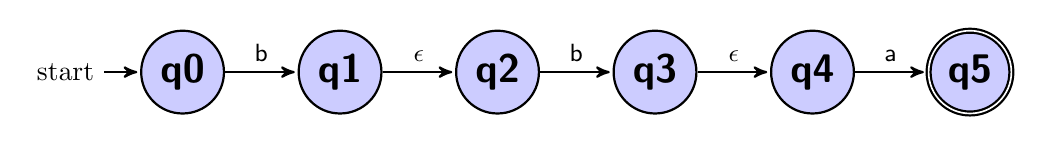
\begin{tikzpicture}[->,>=stealth',shorten >=1pt,auto,node distance=2cm,
  thick,main node/.style={circle,fill=blue!20,draw,font=\sffamily\Large\bfseries}]
  \node[main node, initial] (q0) {q0};
  \node[main node] (q1) [right of =q0] {q1};
  \node[main node] (q2) [right of =q1] {q2};
  \node[main node] (q3) [right of =q2] {q3};
  \node[main node] (q4) [right of =q3] {q4};
  \node[main node, accepting] (q5) [right of =q4] {q5};
  \path[every node/.style={font=\sffamily\small}]
     (q0) edge node [above]{b}(q1)
     (q1) edge node [above]{$\epsilon$}(q2)
     (q2) edge node [above]{b}(q3)
     (q3) edge node [above]{$\epsilon$}(q4)
     (q4) edge node [above]{a}(q5);
  \end{tikzpicture}
\subsection*{bba*}
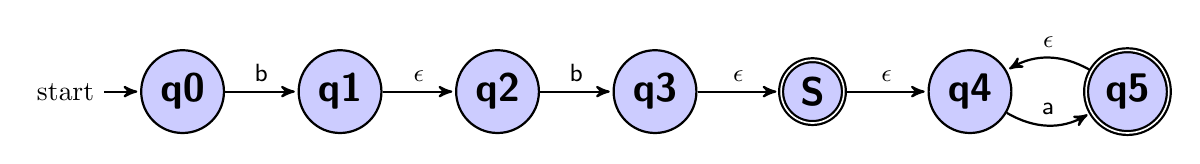
\begin{tikzpicture}[->,>=stealth',shorten >=1pt,auto,node distance=2cm,
  thick,main node/.style={circle,fill=blue!20,draw,font=\sffamily\Large\bfseries}]
  
  \node[main node, initial] (q0) {q0};
  \node[main node] (q1) [right of =q0] {q1};
  \node[main node] (q2) [right of =q1] {q2};
  \node[main node] (q3) [right of =q2] {q3};
  \node[main node, accepting] (S) [right of =q3]{S};
   \node[main node] (q4) [right of =S] {q4};
  \node[main node, accepting] (q5) [right of =q4] {q5};
  \path[every node/.style={font=\sffamily\small}]
  	
     (q0) edge node [above]{b}(q1)
     (q1) edge node [above]{$\epsilon$}(q2)
     (q2) edge node [above]{b}(q3)
     (q3) edge node [above]{$\epsilon$}(S)
     (S) edge node [above]{$\epsilon$}(q4)
     (q4) edge [bend right]  node [above]{a}(q5)
     (q5) edge [bend right] node [above]{$\epsilon$}(q4);
  \end{tikzpicture}
\subsection*{Final}
\begin{tikzpicture}[->,>=stealth',shorten >=1pt,auto,node distance=2cm,
  thick,main node/.style={circle,fill=blue!20,draw,font=\sffamily\Large\bfseries}]
  \node[node] (d){};
  \node[main node, initial] (S)[right of =d,right of =d] {S};
  \node[main node] (q0) [right of =S,below of=S] {q0};
  \node[main node] (q1) [below of =q0] {q1};
  \node[main node] (q2) [below of =q1] {q2};
  \node[main node] (q3) [below of =q2] {q3};
  \node[main node] (q4) [below of =q3] {q4};
  \node[main node] (q5) [below of=q4]{q5};
  \node[main node] (q6) [right of =q5] {q6};
  \node[main node] (q7) [right of =q6] {q7};
  \node[main node, accepting] (q8) [right of =q7] {q8};
  
  \node[main node] (q9)[left of =S,below of=S] {q9};
  \node[main node] (q10) [below of =q9] {q10};
  \node[main node] (q11) [below of =q10] {q11};
  \node[main node] (q12) [below of =q11] {q12};
  \node[main node] (q13) [below of =q12]{q13};
   \node[main node] (q14) [below of =q13] {q14};
  \node[main node] (q15) [below of =q14] {q15};
  \node[main node] (q16) [right of =q15] {q16};
  \node[main node] (q17) [right of =q16] {q17};
   \node[main node] (q18) [right of =q17] {q18};
  \node[main node, accepting] (q19) [right of =q18] {q19};
  \path[every node/.style={font=\sffamily\small}]
  (S) edge node [right]{$\epsilon$} (q0)
  edge node [right]{$\epsilon$} (q9)
     (q0) edge node [right]{a}(q1)
     (q1) edge node [right]{$\epsilon$}(q2)
     (q2) edge node [right]{$\epsilon$}(q3)
     edge [bend right] node [right] {$\epsilon$}(q5)
     (q3) edge [bend right] node [right] {b}(q4)
      (q4) edge [bend right] node [right] {$\epsilon$}(q3)
           edge [bend right] node [right] {$\epsilon$}(q5)
      (q5) edge node [above]{a}(q6)
     (q6) edge node [above]{$\epsilon$}(q7)
     (q7) edge node [above]{a}(q8)
     
     
     (q9) edge node [right]{b}(q10)
     (q10) edge node [right]{$\epsilon$}(q11)
     (q11) edge node [right]{b}(q12)
     (q12) edge node [right]{$\epsilon$}(q13)
     (q13) edge node [right]{$\epsilon$}(q14)
     		edge [bend left]node [right]{$\epsilon$}(q16)
     (q14) edge[bend right] node [right]{a}(q15)
     (q15)edge[bend right] node [right]{$\epsilon$}(q14)
     edge node [below]{$\epsilon$}(q16)
     (q16)edge node [below]{a}(q17)
     (q17)edge node [below]{$\epsilon$}(q18)
     (q18)edge node [below]{b}(q19);
  \end{tikzpicture}
  \section*{Question 5b}
  \subsection*{a}
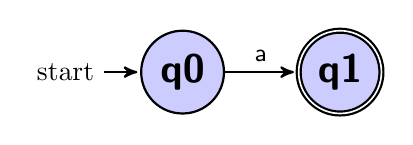
\begin{tikzpicture}[->,>=stealth',shorten >=1pt,auto,node distance=2cm,
  thick,main node/.style={circle,fill=blue!20,draw,font=\sffamily\Large\bfseries}]
  \node[main node, initial] (q0) {q0};
  \node[main node, accepting] (q1) [right of =q0] {q1};
  \path[every node/.style={font=\sffamily\small}]
     (q0) edge node [above]{a}(q1);
  \end{tikzpicture}
\subsection*{b}
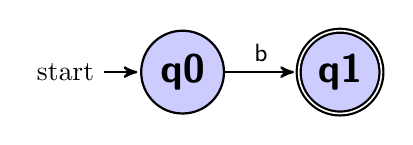
\begin{tikzpicture}[->,>=stealth',shorten >=1pt,auto,node distance=2cm,
  thick,main node/.style={circle,fill=blue!20,draw,font=\sffamily\Large\bfseries}]
  \node[main node, initial] (q0) {q0};
  \node[main node, accepting] (q1) [right of =q0] {q1};
  \path[every node/.style={font=\sffamily\small}]
     (q0) edge node [above]{b}(q1);
  \end{tikzpicture}
  \subsection*{a $\cup$ b}
  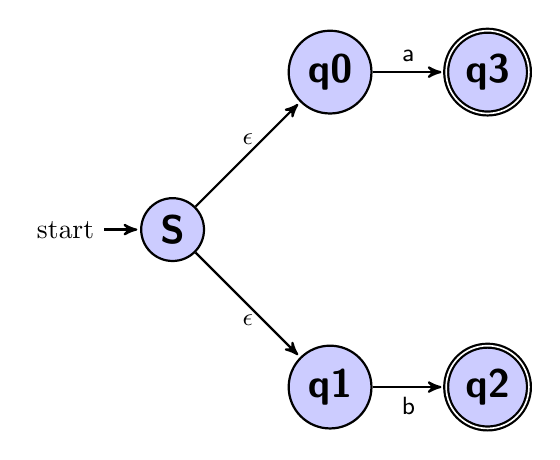
\begin{tikzpicture}[->,>=stealth',shorten >=1pt,auto,node distance=2cm,
  thick,main node/.style={circle,fill=blue!20,draw,font=\sffamily\Large\bfseries}]
  \node[main node, initial] (S) {S};
  \node[main node] (q0) [right of =S, above of =S]{q0};
  \node[main node] (q1) [right of =S, below of =S]{q1};
  \node[main node, accepting] (q2) [right of =q1] {q2};
  \node[main node, accepting] (q3) [right of =q0] {q3};
  \path[every node/.style={font=\sffamily\small}]
     (S) edge node [above]{$\epsilon$}(q0)
         edge node [below]{$\epsilon$}(q1)
     (q0)edge node [above]{a}(q3)
     (q1)edge node [below]{b}(q2);
  \end{tikzpicture}
  \subsection*{(a $\cup$ b)*}
  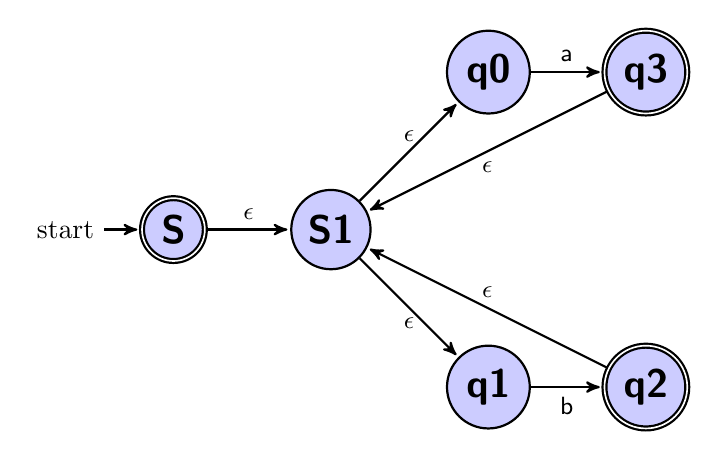
\begin{tikzpicture}[->,>=stealth',shorten >=1pt,auto,node distance=2cm,
  thick,main node/.style={circle,fill=blue!20,draw,font=\sffamily\Large\bfseries}]
  \node[main node, initial, accepting] (S) {S};
  \node[main node] (S1) [right of =S]{S1};
  \node[main node] (q0) [right of =S1, above of =S1]{q0};
  \node[main node] (q1) [right of =S1, below of =S1]{q1};
  \node[main node, accepting] (q2) [right of =q1] {q2};
  \node[main node, accepting] (q3) [right of =q0] {q3};
  \path[every node/.style={font=\sffamily\small}]
  	 (S) edge node [above]{$\epsilon$}(S1)
     (S1) edge node [above]{$\epsilon$}(q0)
         edge node [below]{$\epsilon$}(q1)
     (q0)edge node [above]{a}(q3)
     (q1)edge node [below]{b}(q2)
     (q2)edge node [above]{$\epsilon$}(S1)
     (q3)edge node [below]{$\epsilon$}(S1);
  \end{tikzpicture}
  \subsection*{b(a $\cup$ bb)}
  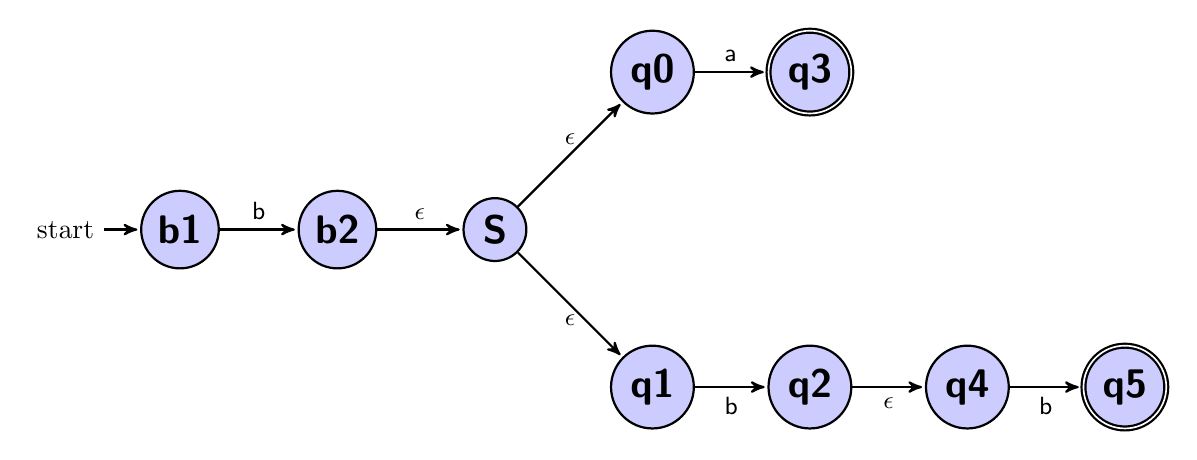
\begin{tikzpicture}[->,>=stealth',shorten >=1pt,auto,node distance=2cm,
  thick,main node/.style={circle,fill=blue!20,draw,font=\sffamily\Large\bfseries}]
  \node[main node, initial] (b1){b1};
  \node[main node] (b2)[right of= b1]{b2};
  \node[main node](S)[right of= b2] {S};
  \node[main node] (q0) [right of =S, above of =S]{q0};
  \node[main node] (q1) [right of =S, below of =S]{q1};
  \node[main node] (q2) [right of =q1] {q2};
  \node[main node, accepting] (q3) [right of =q0] {q3};
  \node[main node] (q4) [right of =q2] {q4};
  \node[main node, accepting] (q5) [right of =q4] {q5};
  \path[every node/.style={font=\sffamily\small}]
  	 (b1)edge node [above]{b}(b2)
     (b2)edge node [above]{$\epsilon$}(S)
     (S) edge node [above]{$\epsilon$}(q0)
         edge node [below]{$\epsilon$}(q1)
     (q0)edge node [above]{a}(q3)
     (q1)edge node [below]{b}(q2)
     (q2)edge node [below]{$\epsilon$}(q4)
     (q4)edge node [below]{b}(q5);
  \end{tikzpicture}
  \subsection*{Final}
  \begin{tikzpicture}[->,>=stealth',shorten >=1pt,auto,node distance=2cm,
  thick,main node/.style={circle,fill=blue!20,draw,font=\sffamily\Large\bfseries}]
  \node (temp);
  \node[main node, initial,accepting] (S)[right of =temp,right of =temp,right of =temp]{S};
  \node[main node] (s1)[below of= S]{s1};
  \node[main node] (s2)[below of= s1]{s2};
  \node[main node] (a1)[right of=s2, below of=s2]{a1};
  \node[main node] (b1)[left of =s2, below of=s2]{b1};
  \node[main node] (a2)[below of=a1]{a2};
  \node[main node] (b2)[below of=b1]{b2};
  \node[main node] (b3)[below of=b2, right of=b2]{b3};
  \node[main node] (b4)[below of=b3]{b4};
  \node[main node] (s3)[below of=b4]{s3};
  \node[main node] (a3)[right of=s3, below of=s3]{a3};
  \node[main node] (b5)[left of =s3, below of=s3]{b5};
  \node[main node,accepting] (a4)[below of=a3]{a4};
  \node[main node] (b6)[below of=b5]{b6};
  \node[main node] (b7)[below of=b6]{b7};
  \node[main node,accepting] (b8)[below of=b7]{b8};
  \path[every node/.style={font=\sffamily\small}]
    (S) edge node [right]{$\epsilon$}(s1)
    (s1)edge node [right]{$\epsilon$}(s2)
    edge [bend right=89]node [left]{$\epsilon$}(b3)
    (s2)edge node [right]{$\epsilon$}(a1)
        edge node [right]{$\epsilon$}(b1)
    (a1)edge node [right]{a}(a2)
    (b1)edge node [right]{b}(b2)
    (a2)edge node [right]{$\epsilon$}(b3)
        edge node [right]{$\epsilon$}(s2)
    (b2)edge node [right]{$\epsilon$}(b3)
        edge node [right]{$\epsilon$}(s2)
    (b3)edge node [right]{b}(b4)
    (b4)edge node [right]{$\epsilon$}(s3)
    (s3)edge node [right]{$\epsilon$}(a3)
        edge node [right]{$\epsilon$}(b5)
    (a3)edge node [right]{a}(a4)
    (a4)edge [bend right=60]node [right]{$\epsilon$}(s1)
    (b5)edge node [right]{b}(b6)
    (b6)edge node [right]{$\epsilon$}(b7)
    (b7)edge node [right]{b}(b8)
    (b8)edge [bend left=80] node [left]{$\epsilon$}(s1);
\end{tikzpicture}
\section*{Question 5c}
\subsection*{\emptyset}
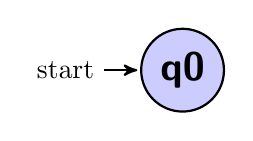
\begin{tikzpicture}[->,>=stealth',shorten >=1pt,auto,node distance=2cm,
  thick,main node/.style={circle,fill=blue!20,draw,font=\sffamily\Large\bfseries}]
  \node[main node, initial] (q0) {q0};
  \end{tikzpicture}
 \subsection*{\emptyset^{*}}
  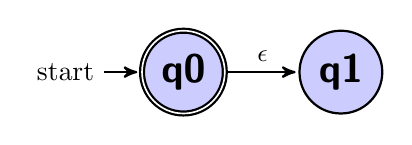
\begin{tikzpicture}[->,>=stealth',shorten >=1pt,auto,node distance=2cm,
  thick,main node/.style={circle,fill=blue!20,draw,font=\sffamily\Large\bfseries}]
  \node[main node, initial, accepting] (q0) {q0};
  \node[main node] (q1) [right of =q0] {q1};
  \path[every node/.style={font=\sffamily\small}]
     (q0) edge node [above]{$\epsilon$}(q1);
  \end{tikzpicture}
\section*{Question 6a}
\begin{itemize}
\item[\textbf{Member}] a
\item[\textbf{Member}] b
\item[\textbf{Non Member}] bba
\item[\textbf{Non Member}] bab
\end{itemize}
\section*{Question 6b}
\begin{itemize}
\item[\textbf{Member}] a
\item[\textbf{Member}] bb
\item[\textbf{Non Member}] b
\item[\textbf{Non Member}] $\epsilon$
\end{itemize}
\newpage
\section*{Question 7}
\begin{itemize}
\item[\textbf{Step 1}] cross out the row of q7 because it is the only state that has out going arrows. Which means it can not be equavalent to any other state.
\item[\textbf{Step 2}] Mark all the (non final state, final state) pairs.

\end{itemize}
\begin{table}[h!t]
\begin{tabular}{c|c|c}
\hline
   tFunction& result & change\\
   %zero
 \hline
 $\delta$(\{q1, q0\}, 0) & \{q0, q1\} &  no mark \\
 $\delta$(\{q1, q0\}, 1) & \{q0, q2\} &  no mark \\
 \hline
 $\delta$(\{q2, q0\}, 0) & \{q3, q1\} &  mark \\
 $\delta$(\{q2, q0\}, 1) & \{q1, q0\} &   \\
 \hline
 $\delta$(\{q4, q0\}, 0) & \{q3, q1\} &  mark \\
 $\delta$(\{q4, q0\}, 1) & \{q0, q1\} &   \\
 \hline
 $\delta$(\{q5, q0\}, 0) & \{q4, q0\} &  mark \\
 $\delta$(\{q5, q0\}, 1) & \{q6, q1\} &  \\
 \hline
 $\delta$(\{q6, q0\}, 0) & \{q0, q1\} &  no mark \\
 $\delta$(\{q6, q0\}, 1) & \{q0, q1\} &  no mark \\
 
 %one
 \hline
 $\delta$(\{q2, q1\}, 0) & \{q3, q0\} &  mark \\
 $\delta$(\{q2, q1\}, 1) & \{q1, q2\} &  \\
 \hline
 $\delta$(\{q4, q1\}, 0) & \{q3, q0\} &  mark \\
 $\delta$(\{q4, q1\}, 1) & \{q5, q2\} &   \\
 \hline
 $\delta$(\{q5, q1\}, 0) & \{q4, q2\} & no mark \\
 $\delta$(\{q5, q1\}, 1) & \{q6, q0\} & no mark \\
 \hline
 $\delta$(\{q6, q1\}, 0) & \{q5, q0\} &  mark \\
 $\delta$(\{q6, q1\}, 1) & \{q6, q2\} &  \\
 
 %two
 \hline
 $\delta$(\{q4, q2\}, 0) & \{q3, q3\} & no mark \\
 $\delta$(\{q4, q2\}, 1) & \{q5, q1\} & no mark   \\
 \hline
 $\delta$(\{q5, q2\}, 0) & \{q6, q3\} & mark \\
 $\delta$(\{q5, q2\}, 1) & \{q4, q1\} & \\
 \hline
 $\delta$(\{q6, q2\}, 0) & \{q6, q1\} &  mark \\
 $\delta$(\{q6, q2\}, 1) & \{q5, q3\} &  \\
 
 %four
 \hline
 $\delta$(\{q5, q4\}, 0) & \{q4, q5\} & mark \\
 $\delta$(\{q5, q4\}, 1) & \{q6, q3\} & \\
 \hline
 $\delta$(\{q6, q4\}, 0) & \{q5, q3\} &  mark \\
 $\delta$(\{q6, q4\}, 1) & \{q6, q5\} &  \\
 \hline
 $\delta$(\{q1, q0\}, 0) & \{q0, q1\} &  no mark \\
 $\delta$(\{q1, q0\}, 1) & \{q0, q2\} &  mark \\
 \hline
\end{tabular}
\end{table}
\begin{table}[h!t]
\begin{tabular}{|c|c|c|c|c|c|c|c|c|}
\hline
    & q0 & q1 & q2 & q3 & q4 & q5 & q6 &q7\\
 \hline
 q0 & -  & -  & -  & -  & -  & -  & -  & -\\
 \hline
 q1 & x  & -  & -  & -  & -  & -  & -  & -\\
 \hline
 q2 & x  & x  & -  & -  & -  & -  & -  & -\\
 \hline
 q3 & x  & x  & x  & -  & -  & -  & -  & -\\
 \hline
 q4 & x  & x  &    & x  & -  & -  & -  & -\\
 \hline
 q5 & x  &    & x  & x  & x  & -  & -  & -\\
 \hline
 q6 &    & x  & x  & x  & x  & x  & -  & -\\
 \hline
 q7 & x  & x  & x  & x  & x  & x  & x  & -\\
 \hline
\end{tabular}
\end{table}
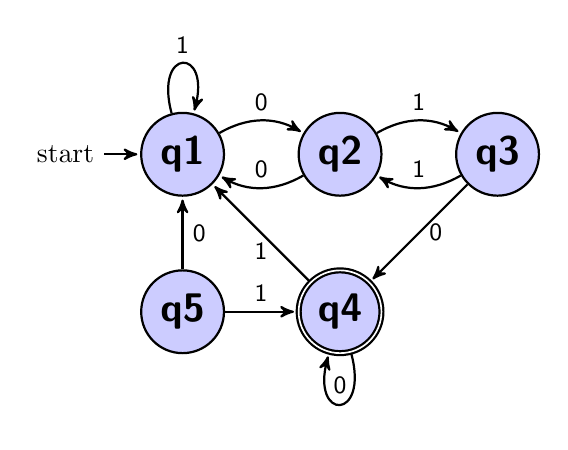
\begin{tikzpicture}[->,>=stealth',shorten >=1pt,auto,node distance=2cm,
  thick,main node/.style={circle,fill=blue!20,draw,font=\sffamily\Large\bfseries}]
  \node[main node, initial] (q1){q1};
  \node[main node] (q2)[right of= q1]{q2};
  \node[main node] (q3)[right of= q2]{q3};
  \node[main node, accepting] (q4)[below of=q2]{q4};
  \node[main node] (q5)[below of=q1]{q5};
  \path[every node/.style={font=\sffamily\small}]
    (q1) edge[loop above] node [above]{1}(q1)
         edge [bend left] node [above] {0}(q2)
    (q2) edge [bend left] node [above] {0}(q1)
         edge [bend left] node [above] {1}(q3)
    (q3) edge [bend left] node [above] {1}(q2)
    		 edge             node [right] {0}(q4)
    (q4) edge             node [below] {1}(q1)
         edge [loop below]node [above] {0}(q4)
    (q5) edge             node [right] {0}(q1)
         edge             node [above] {1}(q4);
\end{tikzpicture}
\end{document}
